\section{Experiments}
\label{experiments}
In mobile voice manipulation applications and in found data cases, it is mandatory to use audio recorded far from the ideal studio conditions, with the possibility of finding background noise.
%
The speaker-adaptive HMM-based paradigm has been found quite robust on mel-cepstrum \cite{karhila_jstsp_14, yamagishi2008robustness} and LSP-based vocoders \cite{yanagisawa2013noise}.
%
Nevertheless, in some vocoding and adaptation techniques noise present in the adaptation data can add background noise and produce distortion in the synthetic speech signal.

A GlottHMM-based speaker-adaptive statistical speech synthesis is built in this project, testing the effects of using noisy data in the adaptation.
%
The different noises included in the adaptation data are: babble noise, factory noise and machine gun noise, with different signal-to-noise ratio (SNR).
%
These noises where artificially added into clean data.
%
The results will be compared to the ones obtained with the STRAIGHT-based system in \cite{karhila_jstsp_14}.

\subsection{Initial Experiments}
\label{experiments_initial}
The use of glottal pulses for HMM-synthesis was originally proposed due to the buzzy voice quality caused by simple excitation \cite{raitio2008hmm}.
%
However, a proper modelling of the glottal pulse shape improves the quality in the case of lower fundamental frequency speakers, while speakers with higher $F_{0}$, such as women, do not benefit from the pulse and the impulse excitation may be adequate for them.
%
This particular behavior is the reason of working with a male average voice model, knowing that glottal inverse filtering approach flaws when synthesizing high-pitched voices.

The first step is testing the performance in analysis-resynthesis of GlottHMM when noisy data is used, in order to see if GlottHMM suffer any huge inconvenient caused by the noise.

\begin{figure}[!htb]
\begin{centering}
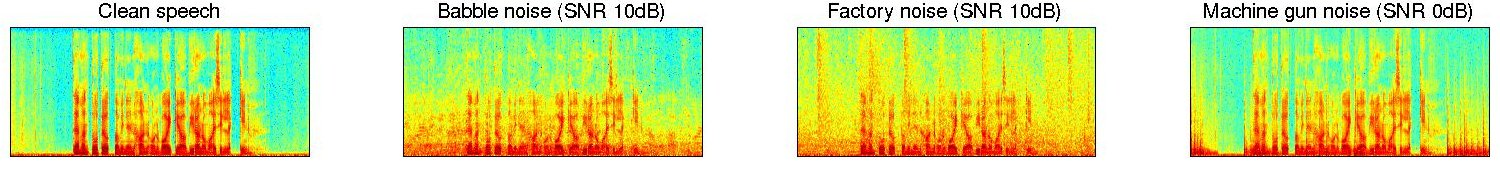
\includegraphics[width=\textwidth]{images/natural_spectra.jpg}
\caption{Natural speech FFT spectra of clean speech, speech with babble noise, factory noise and machine gun noise}
\label{fig:natural_spectra}
\end{centering}
\end{figure}

Figure \ref{fig:natural_spectra} shows the spectra of a natural speech sample in different environmental conditions while Figure \ref{fig:synthetic_spectra} shows the spectra of the same samples resynthesized with GlottHMM.

\begin{figure}[!htb]
\begin{centering}
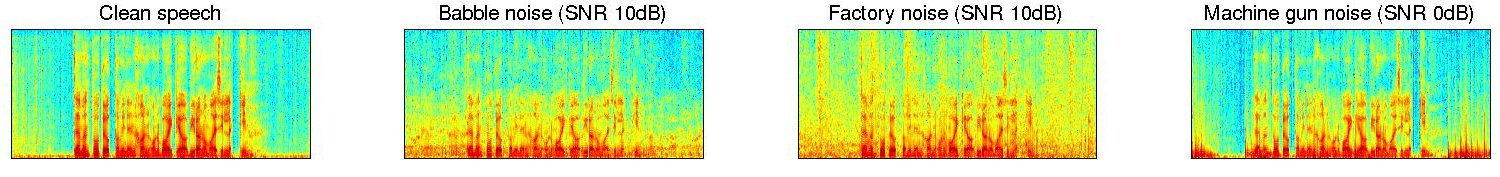
\includegraphics[width=\textwidth]{images/synthetic_spectra.jpg}
\caption{Synthetic speech FFT spectra of clean speech, speech with babble noise, factory noise and machine gun noise after analysis and resynthesis with GlottHMM}
\label{fig:synthetic_spectra}
\end{centering}
\end{figure}

As it can be seen, both the natural and the synthetic spectra has little differences between them.
%
%
After listening to the samples we could conclude that noise was not influencing the regular performance GlottHMM.

Another important issue is finding a correct configuration for GlottHMM.
%
In Appendix \ref{glott_conf_file}, the configuration file needed by GlottHMM can be found.
%
This file has a great amount of options to configure. 
%
However, thanks to previous experiments conducted and the advice of Tuomo Raitio, who developed GlottHMM, the tweaks to make in the configuration file are focused in noise robustness and some voice characteristics.

Some low $F_{0}$ problems were noticed during the first rounds of experiments.
% 
This problems consisted of frames where the voice sounded funny.
%
To find out the details of this issue, a simple $F_{0}$ histogram plotting was made.
%
Figure \ref{fig:f0_histograms} presents the histograms of the voices used to build the average voice model, where low-frequency peaks can be pointed out in some of the voices.

\begin{figure}[!htb]
\begin{centering}
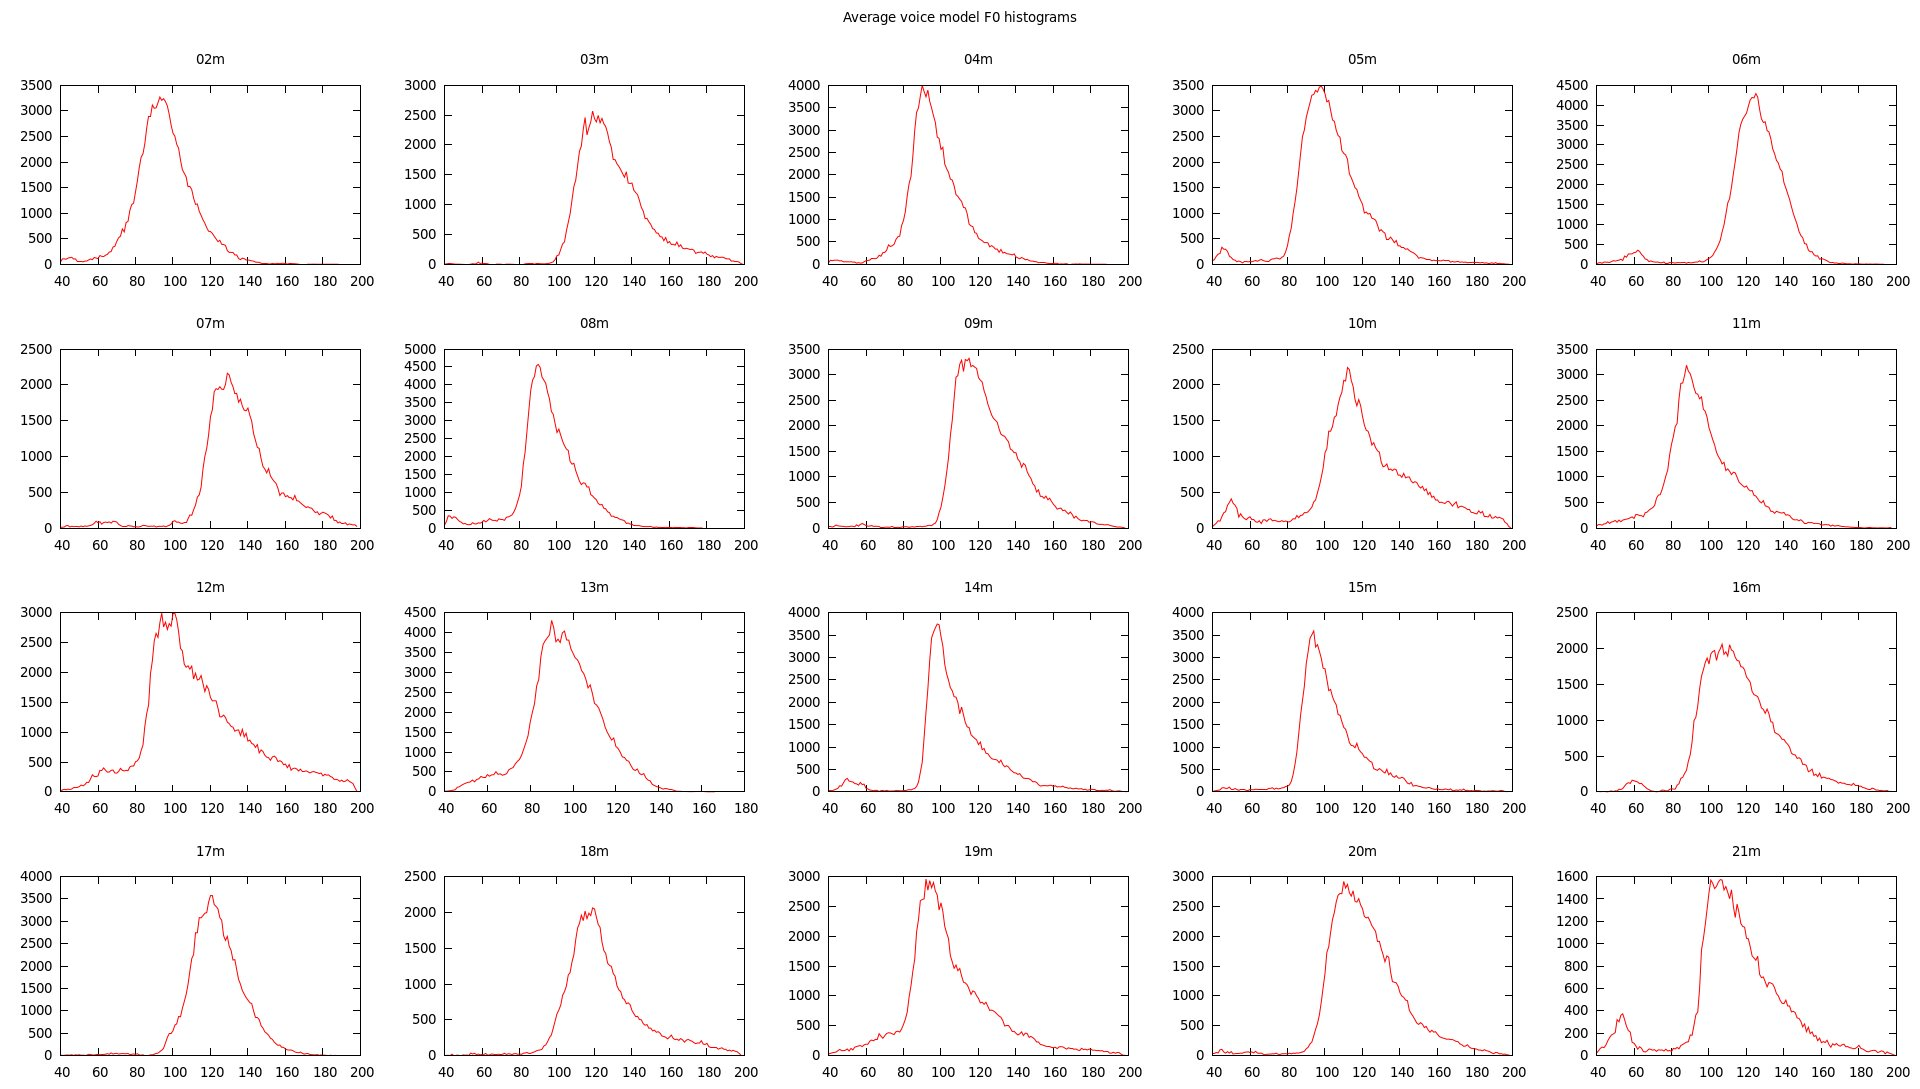
\includegraphics[width=\textwidth]{images/av_model_=conf_f0_histogram.jpg}
\caption{$F_{0}$ histogram of the voices composing the average voice model}
\label{fig:f0_histograms}
\end{centering}
\end{figure}

Solving this problem only required to extract again the features for the voices with low-frequency peaks.
%
These peaks were found around 40-60 Hz in the training data, used in the average voice model, and in the adaptation data.
%
To eliminate them, in the configuration file the $F_{0}$ lower-limit was set to 65 Hz.

The last round of initial experiments conducted aim to find the best combination of the noise reduction parameters shown in Appendix \ref{glott_conf_noise_red}.
%
These experiments consist on analysis and resynthesis of the noisy data varying the parameters in Appendix \ref{glott_conf_noise_red} and carrying out the objective measures described in \ref{evaluation_objective}.
%
